
\pagebreak

\section*{Introduction}

\subsection*{De la nécessaire sécurité des applications web}

\addcontentsline{toc}{section}{Introduction}
%\markboth{Introduction}{} 
Comme TV5 monde en 2015, les pertes des entreprises victimes de cyberattaques se comptent souvent en dizaines de millions d'euros. L'Open Web Application Security Project (\href{https://www.owasp.org}{OWASP}), publie régulièrement la liste des 10 menaces les plus critiques qui concernent les applications web. Une manière de s'en prémunir consiste à pratiquer le hacking web éthique. C'est là qu'entre en scène l'outil Damn Vulnerable Web Application (\href{http://www.dvwa.co.uk}{DVWA}). Il s'agit d'un environnement PHP qui permet de se former à la sécurité des sites web. Le hacker en herbe peut ainsi se former et tester légalement ses compétences sur une application hébergée localement. C'est ce qu'on se propose d'exposer dans ce document.  

\begin{figure}[!h]
	\begin{center}
		\label{10_menaces}
		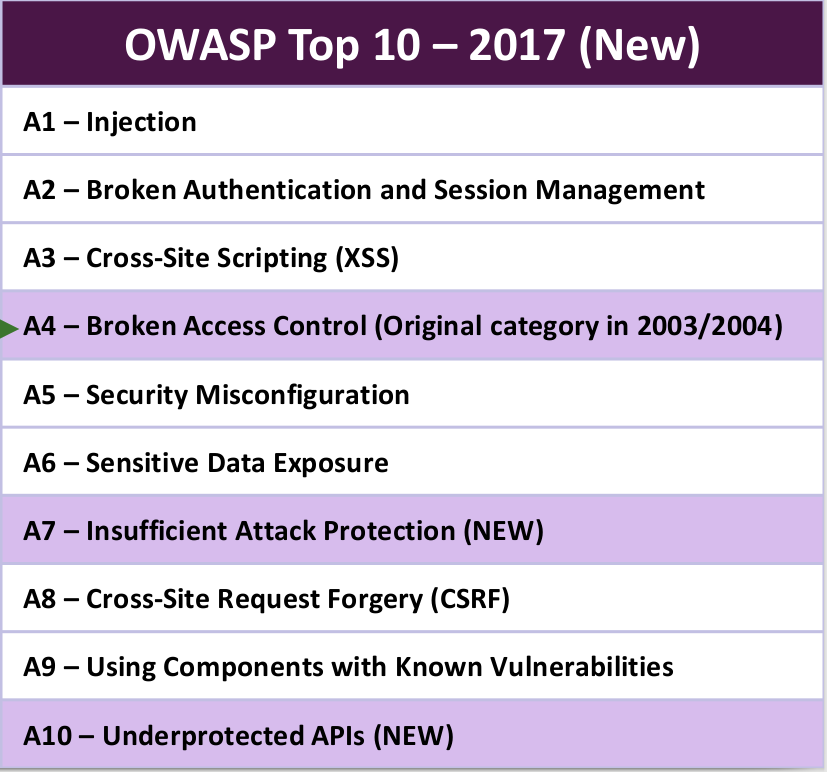
\includegraphics[scale=0.4]{images/10_menaces.png}
		\caption{Le top 10 des menaces web 2017 publiées par l'OWASP}
	\end{center}
\end{figure}

\subsection*{Mise en place d'une plateforme de test}

Une solution possible consiste à installer la distribution kali et le site web DVWA sur une machine virtuelle VirtualBox. On utilisera PHP 5, plutôt que PHP 7, comme demandé dans la documentation d'installation.
Il suffit ensuite de modifier la configuration réseau NAT de la machine virtuelle en "accès par pont" pour pouvoir accéder au site DVWA à partir de la machine hôte.
La commande \texttt{hostname -I} sur la machine virtuelle fournit son adresse IP, par exemple 192.168.1.8. Il ne reste plus qu'à se connecter via firefox
au site dvwa grâce à l'URL \path{http://192.168.1.8/dvwa/}. Il est également possible d'utiliser DVWA directement sur la machine virtuelle via l'adresse \path{http://localhost/dvwa}. Les deux méthodes seront utilisées dans ce document. Le login par défaut est admin/password.

 \begin{figure}[!h]
 	\begin{center}
 		\label{}
 		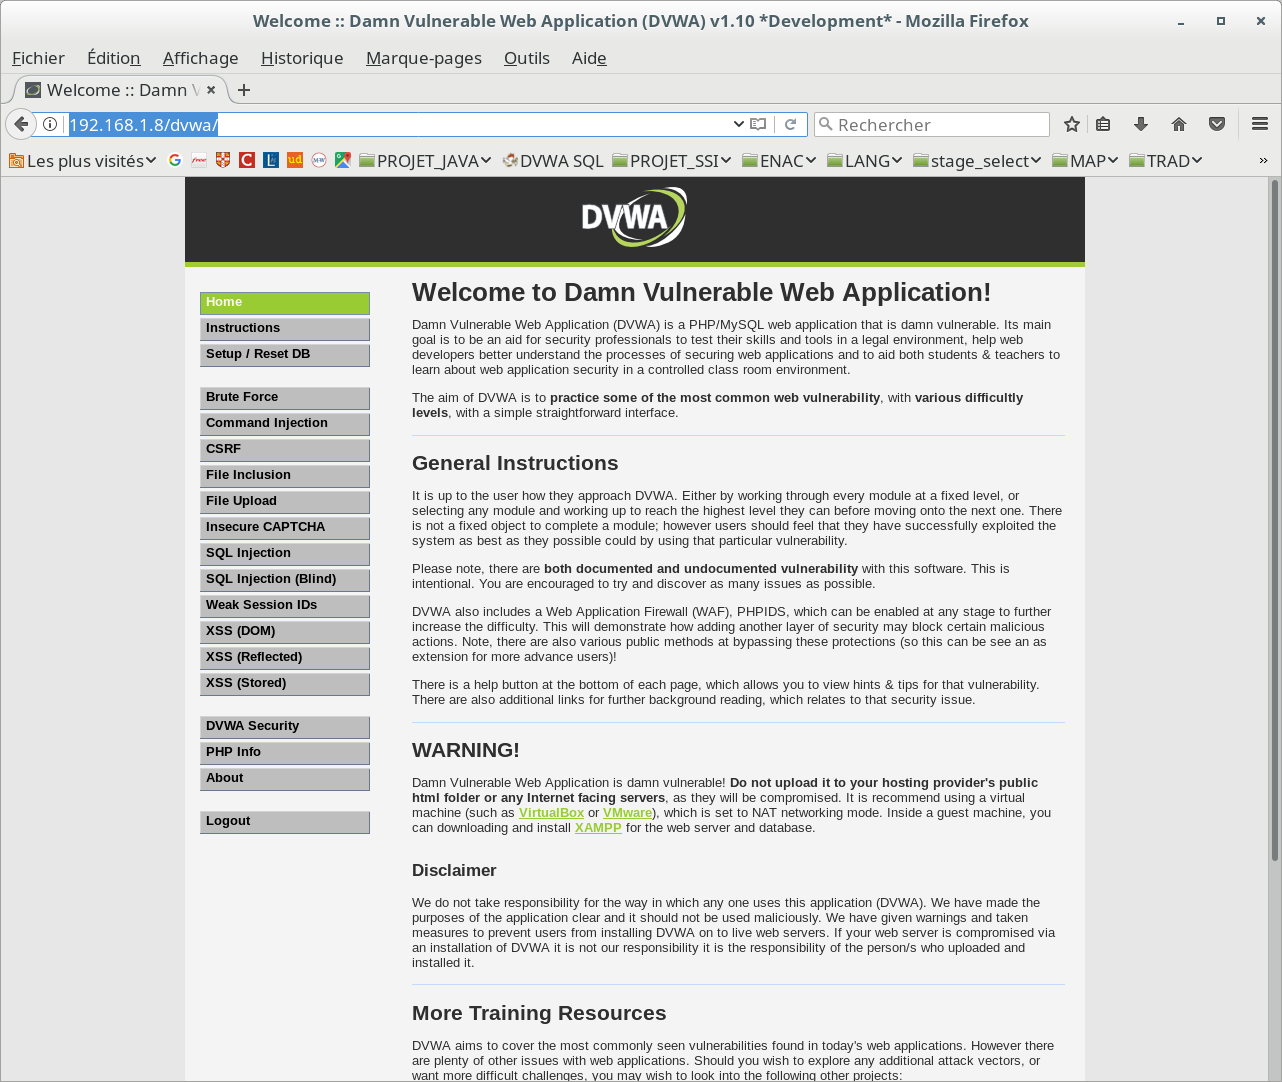
\includegraphics[scale=\scaledvwa]{images/dvwa.png}
 		\caption{Accès à DVWA à partir du navigateur de la machine hôte. Le site web DVWA est installé sur une machine virtuelle kali linux.}
 	\end{center}
 \end{figure}


\clearpage